\documentclass[14pt,a4paper]{scrartcl}
\renewcommand{\sfdefault}{cmr}

\usepackage[utf8]{inputenc}
\usepackage[english,russian]{babel}

\usepackage{indentfirst}
\usepackage{graphicx}
\usepackage{misccorr}
\usepackage{amsmath}
\usepackage{amssymb}
\usepackage{amsfonts}

\usepackage{enumitem}
\usepackage{soul}
\usepackage{soulutf8}


\begin{document}
	\begin{flushright}
	\textbf{Билеты по теоретической неорганической химии\\
		Факультет химии, 1 курс}
\end{flushright}  	

\section{3 Модуль}

%IMPORT TEX FILE FOR EACH QUESTION

\subsection{Вопрос 1}

%NO PREAMBLE, NO \begin{document} or \usepackage here !
Вопрос 1, бла-бла-бла...

\begin{itemize}
\item раз
\item два
\item три
\end{itemize}

\begin{figure}[htp]
\centering
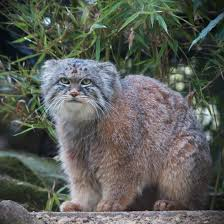
\includegraphics[scale=1.00]{/home/someanonimcoder/TeX/tic_summer/images/manul.jpeg}
\caption{eine manulle...}
\label{}
\end{figure}


%\subsection{Вопрос 2}
%
%NO PREAMBLE, NO \begin{document} or \usepackage here !
\subsection{Симметрия расщеплений d-орбиталей. Энергия стабилизации кристаллическим полем.}

\subsubsection*{ЭСКП}

Энергия стабилизации кристаллическим полем (ЭСКП) — энергия электронной конфигурации иона переходного металла относительно средней энергии орбиталей. Стабилизация возникает вследствие того, что в поле лигандов энергетический уровень некоторых орбиталей ниже, чем в гипотетическом сферическом поле, в котором на все пять d-орбиталей действует одинаковая сила отталкивания, и все d-орбитали вырождены. Например, в октаэдрическом случае уровень $t_{2g}$ ниже, чем средний уровень в сферическом поле. Следовательно, если в данных орбиталях находятся электроны, то ион металла более стабилен в поле лигандов относительно сферического поля. Наоборот, энергетический уровень орбиталей $e_g$ выше среднего, и электроны, находящиеся в них, уменьшают стабилизацию.


\begin{figure}[H]
\centering
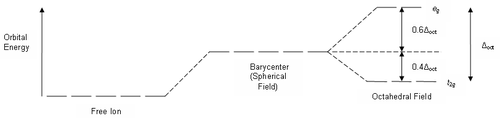
\includegraphics[scale=.750]{/home/someanonimcoder/TeX/tic_summer/images/CFSE.png}
\caption{диарграмма расщепления}
\label{}
\end{figure}

\subsubsection*{Типичные расщепления}

Для получения этих расщеплений обычно рассмтривают изолированные орбитали d, к которым "придвигают" 8 заместителей, получая октаэдрическое расщепление, от которого потом постепенно "убирают" заместители.

\begin{figure}[H]%
    \centering
    \subfloat[катринка]{{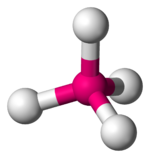
\includegraphics[width=5cm]{images/tetrahedr.png} }}%
    \qquad
    \subfloat[диаграмма орбиталей]{{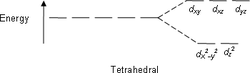
\includegraphics[width=5cm]{images/tetrahedr_orb.png} }}%
    \label{fig:example}%
        \caption{Тетраэдрическое расщепление}
\end{figure}



\begin{figure}[H]%
    \centering
    \subfloat[катринка]{{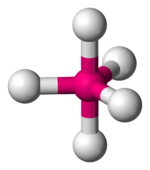
\includegraphics[width=5cm]{images/trig-bip.png} }}%
    \qquad
    \subfloat[диаграмма орбиталей]{{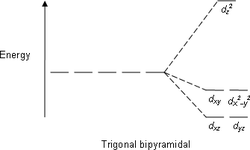
\includegraphics[width=5cm]{images/trig-bip_orb.png} }}%
    \label{fig:example}%
    \caption{Тригонально-бипирамидальное расщепление}
\end{figure}


\begin{figure}[H]%
    \centering
    \subfloat[катринка]{{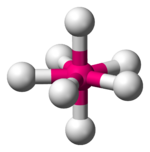
\includegraphics[width=5cm]{images/pent-bip.png} }}%
    \qquad
    \subfloat[диаграмма орбиталей]{{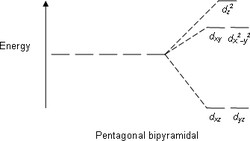
\includegraphics[width=5cm]{images/pent-bip_orb.png} }}%
    \label{fig:example}%
    \caption{Пентагонально-бипирамидальное расщепление}
\end{figure}


\begin{figure}[H]%
    \centering
    \subfloat[катринка]{{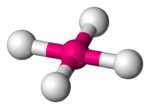
\includegraphics[width=5cm]{images/planar.png} }}%
    \qquad
    \subfloat[диаграмма орбиталей]{{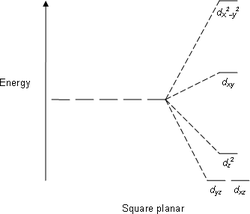
\includegraphics[width=5cm]{images/planar_orb.png} }}%
    \label{fig:example}%
    \caption{Плоскоквадрвтное расщепление}
\end{figure}

\begin{figure}[H]%
    \centering
    \subfloat[катринка]{{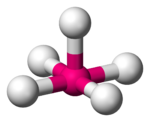
\includegraphics[width=5cm]{images/sq-piram.png} }}%
    \qquad
    \subfloat[диаграмма орбиталей]{{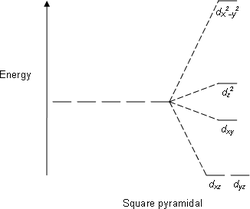
\includegraphics[width=5cm]{images/sq-piram_orb.png} }}%
    \label{fig:example}%
    \caption{Квадратно-пирамидальное расщепление}
\end{figure}

\begin{figure}[H]%
    \centering
    \subfloat[катринка]{{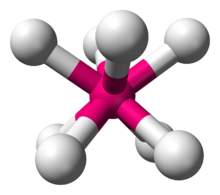
\includegraphics[width=5cm]{images/sq-antipr.png} }}%
    \qquad
    \subfloat[диаграмма орбиталей]{{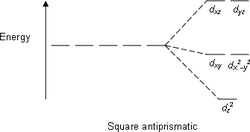
\includegraphics[width=5cm]{images/sq-antipr_orb.png} }}%
    \label{fig:example}%
    \caption{Квадратно-антипризматическое расщепление}
\end{figure}







%...

\section{4 Модуль}

%\subsection{Вопрос 1}
%
%NO PREAMBLE, NO \begin{document} or \usepackage here !
\subsection{Симметрия расщеплений d-орбиталей. Энергия стабилизации кристаллическим полем.}

\subsubsection*{ЭСКП}

Энергия стабилизации кристаллическим полем (ЭСКП) — энергия электронной конфигурации иона переходного металла относительно средней энергии орбиталей. Стабилизация возникает вследствие того, что в поле лигандов энергетический уровень некоторых орбиталей ниже, чем в гипотетическом сферическом поле, в котором на все пять d-орбиталей действует одинаковая сила отталкивания, и все d-орбитали вырождены. Например, в октаэдрическом случае уровень $t_{2g}$ ниже, чем средний уровень в сферическом поле. Следовательно, если в данных орбиталях находятся электроны, то ион металла более стабилен в поле лигандов относительно сферического поля. Наоборот, энергетический уровень орбиталей $e_g$ выше среднего, и электроны, находящиеся в них, уменьшают стабилизацию.


\begin{figure}[H]
\centering
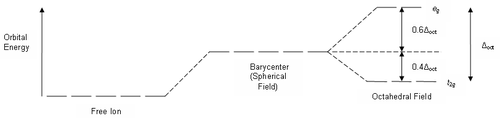
\includegraphics[scale=.750]{/home/someanonimcoder/TeX/tic_summer/images/CFSE.png}
\caption{диарграмма расщепления}
\label{}
\end{figure}

\subsubsection*{Типичные расщепления}

Для получения этих расщеплений обычно рассмтривают изолированные орбитали d, к которым "придвигают" 8 заместителей, получая октаэдрическое расщепление, от которого потом постепенно "убирают" заместители.

\begin{figure}[H]%
    \centering
    \subfloat[катринка]{{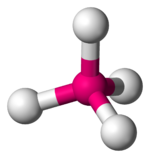
\includegraphics[width=5cm]{images/tetrahedr.png} }}%
    \qquad
    \subfloat[диаграмма орбиталей]{{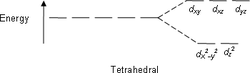
\includegraphics[width=5cm]{images/tetrahedr_orb.png} }}%
    \label{fig:example}%
        \caption{Тетраэдрическое расщепление}
\end{figure}



\begin{figure}[H]%
    \centering
    \subfloat[катринка]{{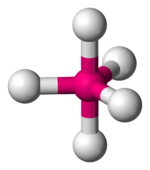
\includegraphics[width=5cm]{images/trig-bip.png} }}%
    \qquad
    \subfloat[диаграмма орбиталей]{{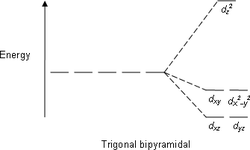
\includegraphics[width=5cm]{images/trig-bip_orb.png} }}%
    \label{fig:example}%
    \caption{Тригонально-бипирамидальное расщепление}
\end{figure}


\begin{figure}[H]%
    \centering
    \subfloat[катринка]{{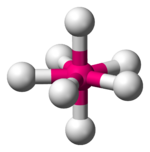
\includegraphics[width=5cm]{images/pent-bip.png} }}%
    \qquad
    \subfloat[диаграмма орбиталей]{{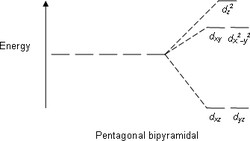
\includegraphics[width=5cm]{images/pent-bip_orb.png} }}%
    \label{fig:example}%
    \caption{Пентагонально-бипирамидальное расщепление}
\end{figure}


\begin{figure}[H]%
    \centering
    \subfloat[катринка]{{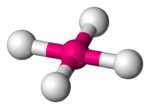
\includegraphics[width=5cm]{images/planar.png} }}%
    \qquad
    \subfloat[диаграмма орбиталей]{{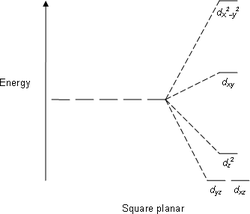
\includegraphics[width=5cm]{images/planar_orb.png} }}%
    \label{fig:example}%
    \caption{Плоскоквадрвтное расщепление}
\end{figure}

\begin{figure}[H]%
    \centering
    \subfloat[катринка]{{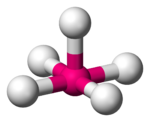
\includegraphics[width=5cm]{images/sq-piram.png} }}%
    \qquad
    \subfloat[диаграмма орбиталей]{{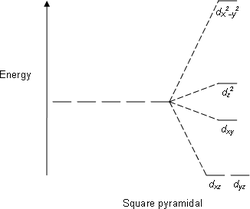
\includegraphics[width=5cm]{images/sq-piram_orb.png} }}%
    \label{fig:example}%
    \caption{Квадратно-пирамидальное расщепление}
\end{figure}

\begin{figure}[H]%
    \centering
    \subfloat[катринка]{{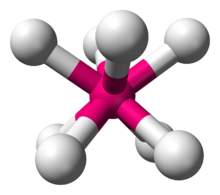
\includegraphics[width=5cm]{images/sq-antipr.png} }}%
    \qquad
    \subfloat[диаграмма орбиталей]{{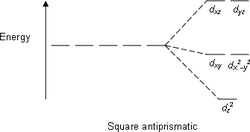
\includegraphics[width=5cm]{images/sq-antipr_orb.png} }}%
    \label{fig:example}%
    \caption{Квадратно-антипризматическое расщепление}
\end{figure}







%\subsection{Вопрос 2}
%
%NO PREAMBLE, NO \begin{document} or \usepackage here !
\subsection{Симметрия расщеплений d-орбиталей. Энергия стабилизации кристаллическим полем.}

\subsubsection*{ЭСКП}

Энергия стабилизации кристаллическим полем (ЭСКП) — энергия электронной конфигурации иона переходного металла относительно средней энергии орбиталей. Стабилизация возникает вследствие того, что в поле лигандов энергетический уровень некоторых орбиталей ниже, чем в гипотетическом сферическом поле, в котором на все пять d-орбиталей действует одинаковая сила отталкивания, и все d-орбитали вырождены. Например, в октаэдрическом случае уровень $t_{2g}$ ниже, чем средний уровень в сферическом поле. Следовательно, если в данных орбиталях находятся электроны, то ион металла более стабилен в поле лигандов относительно сферического поля. Наоборот, энергетический уровень орбиталей $e_g$ выше среднего, и электроны, находящиеся в них, уменьшают стабилизацию.


\begin{figure}[H]
\centering
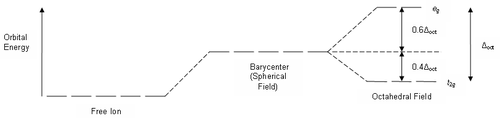
\includegraphics[scale=.750]{/home/someanonimcoder/TeX/tic_summer/images/CFSE.png}
\caption{диарграмма расщепления}
\label{}
\end{figure}

\subsubsection*{Типичные расщепления}

Для получения этих расщеплений обычно рассмтривают изолированные орбитали d, к которым "придвигают" 8 заместителей, получая октаэдрическое расщепление, от которого потом постепенно "убирают" заместители.

\begin{figure}[H]%
    \centering
    \subfloat[катринка]{{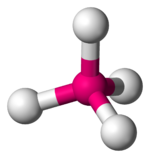
\includegraphics[width=5cm]{images/tetrahedr.png} }}%
    \qquad
    \subfloat[диаграмма орбиталей]{{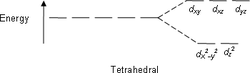
\includegraphics[width=5cm]{images/tetrahedr_orb.png} }}%
    \label{fig:example}%
        \caption{Тетраэдрическое расщепление}
\end{figure}



\begin{figure}[H]%
    \centering
    \subfloat[катринка]{{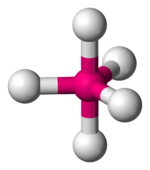
\includegraphics[width=5cm]{images/trig-bip.png} }}%
    \qquad
    \subfloat[диаграмма орбиталей]{{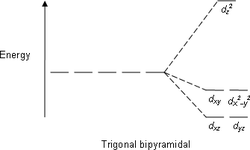
\includegraphics[width=5cm]{images/trig-bip_orb.png} }}%
    \label{fig:example}%
    \caption{Тригонально-бипирамидальное расщепление}
\end{figure}


\begin{figure}[H]%
    \centering
    \subfloat[катринка]{{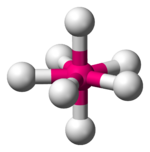
\includegraphics[width=5cm]{images/pent-bip.png} }}%
    \qquad
    \subfloat[диаграмма орбиталей]{{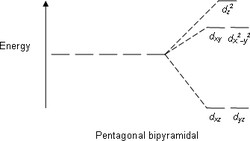
\includegraphics[width=5cm]{images/pent-bip_orb.png} }}%
    \label{fig:example}%
    \caption{Пентагонально-бипирамидальное расщепление}
\end{figure}


\begin{figure}[H]%
    \centering
    \subfloat[катринка]{{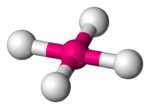
\includegraphics[width=5cm]{images/planar.png} }}%
    \qquad
    \subfloat[диаграмма орбиталей]{{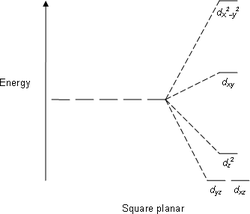
\includegraphics[width=5cm]{images/planar_orb.png} }}%
    \label{fig:example}%
    \caption{Плоскоквадрвтное расщепление}
\end{figure}

\begin{figure}[H]%
    \centering
    \subfloat[катринка]{{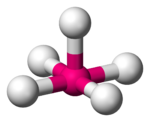
\includegraphics[width=5cm]{images/sq-piram.png} }}%
    \qquad
    \subfloat[диаграмма орбиталей]{{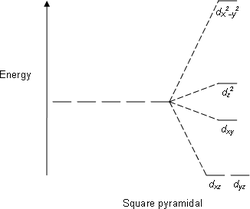
\includegraphics[width=5cm]{images/sq-piram_orb.png} }}%
    \label{fig:example}%
    \caption{Квадратно-пирамидальное расщепление}
\end{figure}

\begin{figure}[H]%
    \centering
    \subfloat[катринка]{{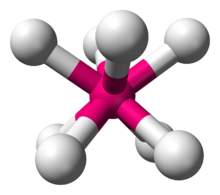
\includegraphics[width=5cm]{images/sq-antipr.png} }}%
    \qquad
    \subfloat[диаграмма орбиталей]{{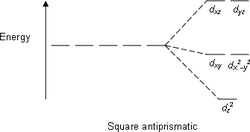
\includegraphics[width=5cm]{images/sq-antipr_orb.png} }}%
    \label{fig:example}%
    \caption{Квадратно-антипризматическое расщепление}
\end{figure}






%\subsection{Вопрос 3}
%\subsection{Сильное и слабое кристаллическое поле. Магнитные и спектральные свойства комплексных соединений переходных металлов}

 Лиганды делятся на две группы – сильного поля, которые расщепляют сильно-низкоспиновые комплексы, и лиганды слабого поля-высокоспиновые комплексы, которые расщепляют слабо. 
 
Интенсивность поля возрастает в следующем ряду:
 
\begin{figure}[H]
\centering
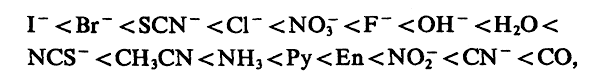
\includegraphics[scale=.600]{images/spectrochem_row.png}
\end{figure}
 
 \subsubsection{Октаэдрическое поле}
 
 \begin{figure}[htp]
\centering
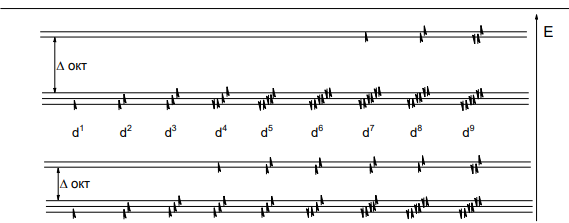
\includegraphics[scale=1.00]{images/electrones.png}
\end{figure} схема заполнения электронов представлена на картинке

 \begin{itemize}
 \item для $d^1-d^3$ ситуация не зависит от расщепления \item для $d^4$ ситуация меняется есть два варианта: для слабого(нижняя диаграмма) расщепления разница в энергии невелика и электроны остаются неспаренными. Образуются 4 неспаренных электрона  для сильного расщепления разница в энергии уровней больше чем энергии спаривания, поэтому получается выигрыш в энергии, когда электрон опускается вниз и спариваются \item для $d^5$ в низкоспиновом комплексе 2 спаренных электрона и 1 неспаренный в высокоспиновом комплексе пять неспаренных электронов для $d^6$ в низкоспиновом комплексе получится полностью заполненные $d_{xz}$,$d_{xy}$,$d_{yz}$ орбитали-диамагнитный комплекс в высокоспиновом комплексе 4 неспаренных электрона 
 \item для $d^7$ в низкоспиновом комплексе 1 неспаренный электрон в высокоспиновом комплексе 3 неспаренных электрона 
 \item для $d^8$-$d^9$ в низкоспиновом комплексе и в высокоспиновом комплексе будут одинаковые картины- по 2(для $d^8$) и 3( для $d^9$) электронов 
 \end{itemize}

\subsubsection*{Тетраэдрическое поле}
тетраэрдрические комплексы формируются только лиганды со слабым полем(высокоспиновые)-почему? потому что $0.5\Delta_{oct}=\Delta_{tetr}$ ( расщепление мало) и спариваться электронам не нужно

а почему расщепление меньше?
\begin{itemize}
\item расстояние до лигандов в тетраэдрическом поле больше, взаимодействие хуже 
\item количество лигандов меньше, чем в окаэдрическом поле и поэтому отталкивание меньше энергия спаривания электронов ($P$) больше, чем $10D_q$ и первые 5 электронов заполняют по одному пять орбиталей и шестой(и последующие) электроны с обратным спином дополняют каждую орбитали. 
\end{itemize}

\subsubsection{магнитные свойства}
 магнитный момент у низкоспиновых меньше, так как электроны спариваются, а не переходят на другие уровни 
$$\mu=2\sqrt{s(s+1)}=\sqrt{n(n+2)}$$ 

s-суммарный спин 

n-число неспаренных электронов 

\subsubsection{Спектральные свойства}
 В зависимости от лигандов комплекс имеет разные цвета. При замещении лиганда изменяется не только число неспаренных электронов, но еще и цвет. В случае высокоспинового комплекса энергия расщепления меньше($E=h\nu$), следовательно частота перехода с $d_{xy},d_{xz},d_{yz}$ на $d_z^2$ , $d_x^2-d_y^2$ меньше, а длина волны поглощаемого цвета больше В случае низкоспинового комплекса ситуация обратная, энергия расщепления больше($E=h\nu$), следовательно частота перехода сс $d_{xy},d_{xz},d_{yz}$ на $d_z^2$ , $d_x^2-d_y^2$ больше, а длина волны поглощаемого цвета меньше (будет поглощать более коротковолновые волны) \begin{figure}[htp]
 
\subsubsection{Соответствие частот и цветов}
\centering
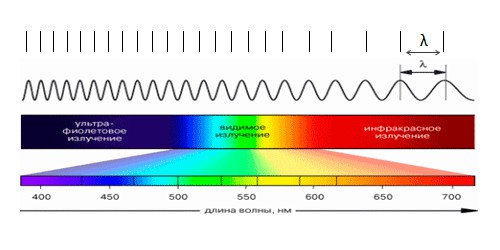
\includegraphics[scale=.750]{images/spectre.jpg}
\end{figure}
 
 



\end{document}
